\documentclass[10pt]{article}
\usepackage[margin=1.7cm]{geometry}
\usepackage[T1]{fontenc}
\usepackage[utf8]{inputenc}
\usepackage{lmodern}
\usepackage{titlesec}
\usepackage{enumitem}
\usepackage{parskip}
\usepackage[table]{xcolor}
\usepackage{graphicx}
\usepackage{tabularx}
\usepackage{array}
\usepackage{booktabs}
\usepackage{hyperref}
\usepackage{fancyhdr}
\usepackage{textcomp}

\definecolor{accent}{RGB}{0,74,124}
\definecolor{head}{RGB}{211,224,229}
\definecolor{soft}{RGB}{244,247,249}
\definecolor{high}{RGB}{246,194,154}
\definecolor{med}{RGB}{252,240,180}

\titleformat{\section}{\large\bfseries\color{accent}}{\thesection.}{0.5em}{}
\titlespacing*{\section}{0pt}{8pt}{3pt}
\titleformat{\subsection}[runin]{\normalsize\bfseries\color{accent}}{}{0pt}{}[.]
\titlespacing*{\subsection}{0pt}{5pt}{0.6em}
\newcommand{\subhead}[1]{\par\vspace{4pt}{\normalsize\bfseries\color{accent}#1}\par\vspace{2pt}}

\setlength{\parskip}{5pt}
\setlist[itemize]{topsep=1pt, itemsep=2pt, leftmargin=*}
\renewcommand{\arraystretch}{1.25}
\newcolumntype{Y}{>{\raggedright\arraybackslash}X}

\pagestyle{fancy}
\fancyhf{}
\renewcommand{\headrulewidth}{0pt}
\cfoot{\small\thepage}

\hypersetup{colorlinks=true, urlcolor=accent, linkcolor=accent,
  pdftitle={Nadhir - Solution Blueprint (AOTN Phase 2.1)}, pdfauthor={}, pdfcreator={}}

\begin{document}

{\small\color{accent}\textbf{AOTN CHALLENGE · TSYP 14 · PHASE 2.1}}

\vspace{-2pt}
{\LARGE\bfseries\color{accent}Solution Blueprint}

\vspace{2pt}
\textbf{Team name:} The Architects \quad
\textbf{Student Branch:} IEEE ENSI SB \quad
\textbf{Solution name:} Nadhir

\vspace{-2pt}
\noindent{\color{accent}\rule{\linewidth}{0.8pt}}

%==================================================================
\section{The Solution}

\subsection{In one sentence}
Nadhir is a low-cost box that uses a camera and a microphone to watch the existing dials, alarm lamps and siren of MT/BT transformer substations in Tunisian factories, and alerts the right people by SMS and voice call before a slow drift turns into a fire, without touching the certified installation.

\subsection{Main user}
The \textbf{on-call qualified electrician (\emph{habilité})} responsible for the substation: the only person allowed to enter the room, yet unable to watch it continuously.
\emph{Secondary users:} the \textbf{night/weekend security guard}, who is on site but not allowed in the room and receives simple alerts, and the \textbf{maintenance and plant managers}, who are the escalation contacts and review the decision log.

\subsection{Key features}
\begin{itemize}
\item \textbf{Touch-nothing monitoring.} A camera reads the existing dials and alarm lamps (where present) and a microphone recognises the existing siren. Nothing is wired to the transformer, so there is nothing to re-certify.
\item \textbf{Trend detection and two alert levels.} Readings are checked against limits and their trend, with an estimate of the time left before a limit is reached. A slow drift raises \textbf{WATCH}; a limit reached, or two signals agreeing (dial + lamp or siren), raises \textbf{INTERVENE NOW}. Anomaly detection is added once enough history has been collected.
\item \textbf{Alerts that reach a person.} INTERVENE NOW goes to the electrician and the guard at the same time by SMS and push. The guard needs no app: they reply ``1'' or ``2'' by SMS. With no acknowledgement in 5 minutes, Nadhir places a voice call, then escalates to the maintenance manager and the plant manager. 4G is the main channel; a 2G module on a different operator sends SMS and voice calls if 4G is down.
\item \textbf{Self-monitoring.} An unreadable dial produces a ``check needed'' message, never a false value. A heartbeat to a cloud watchdog sends \textbf{SYSTEM OFFLINE} if the box goes silent, and the built-in hardware watchdog restarts the box if its software freezes.
\item \textbf{Decision log and continuous learning.} Every alert is recorded with who was notified, when they acknowledged, the decision taken and the verified outcome, and reviewed by the managers the next morning. These verified outcomes are labelled examples: they are used to retune each site's thresholds and cut false alarms, and later to train the anomaly-detection model, so Nadhir improves from what actually happened rather than just storing history.
\end{itemize}

%==================================================================
\section{How It Works}

\noindent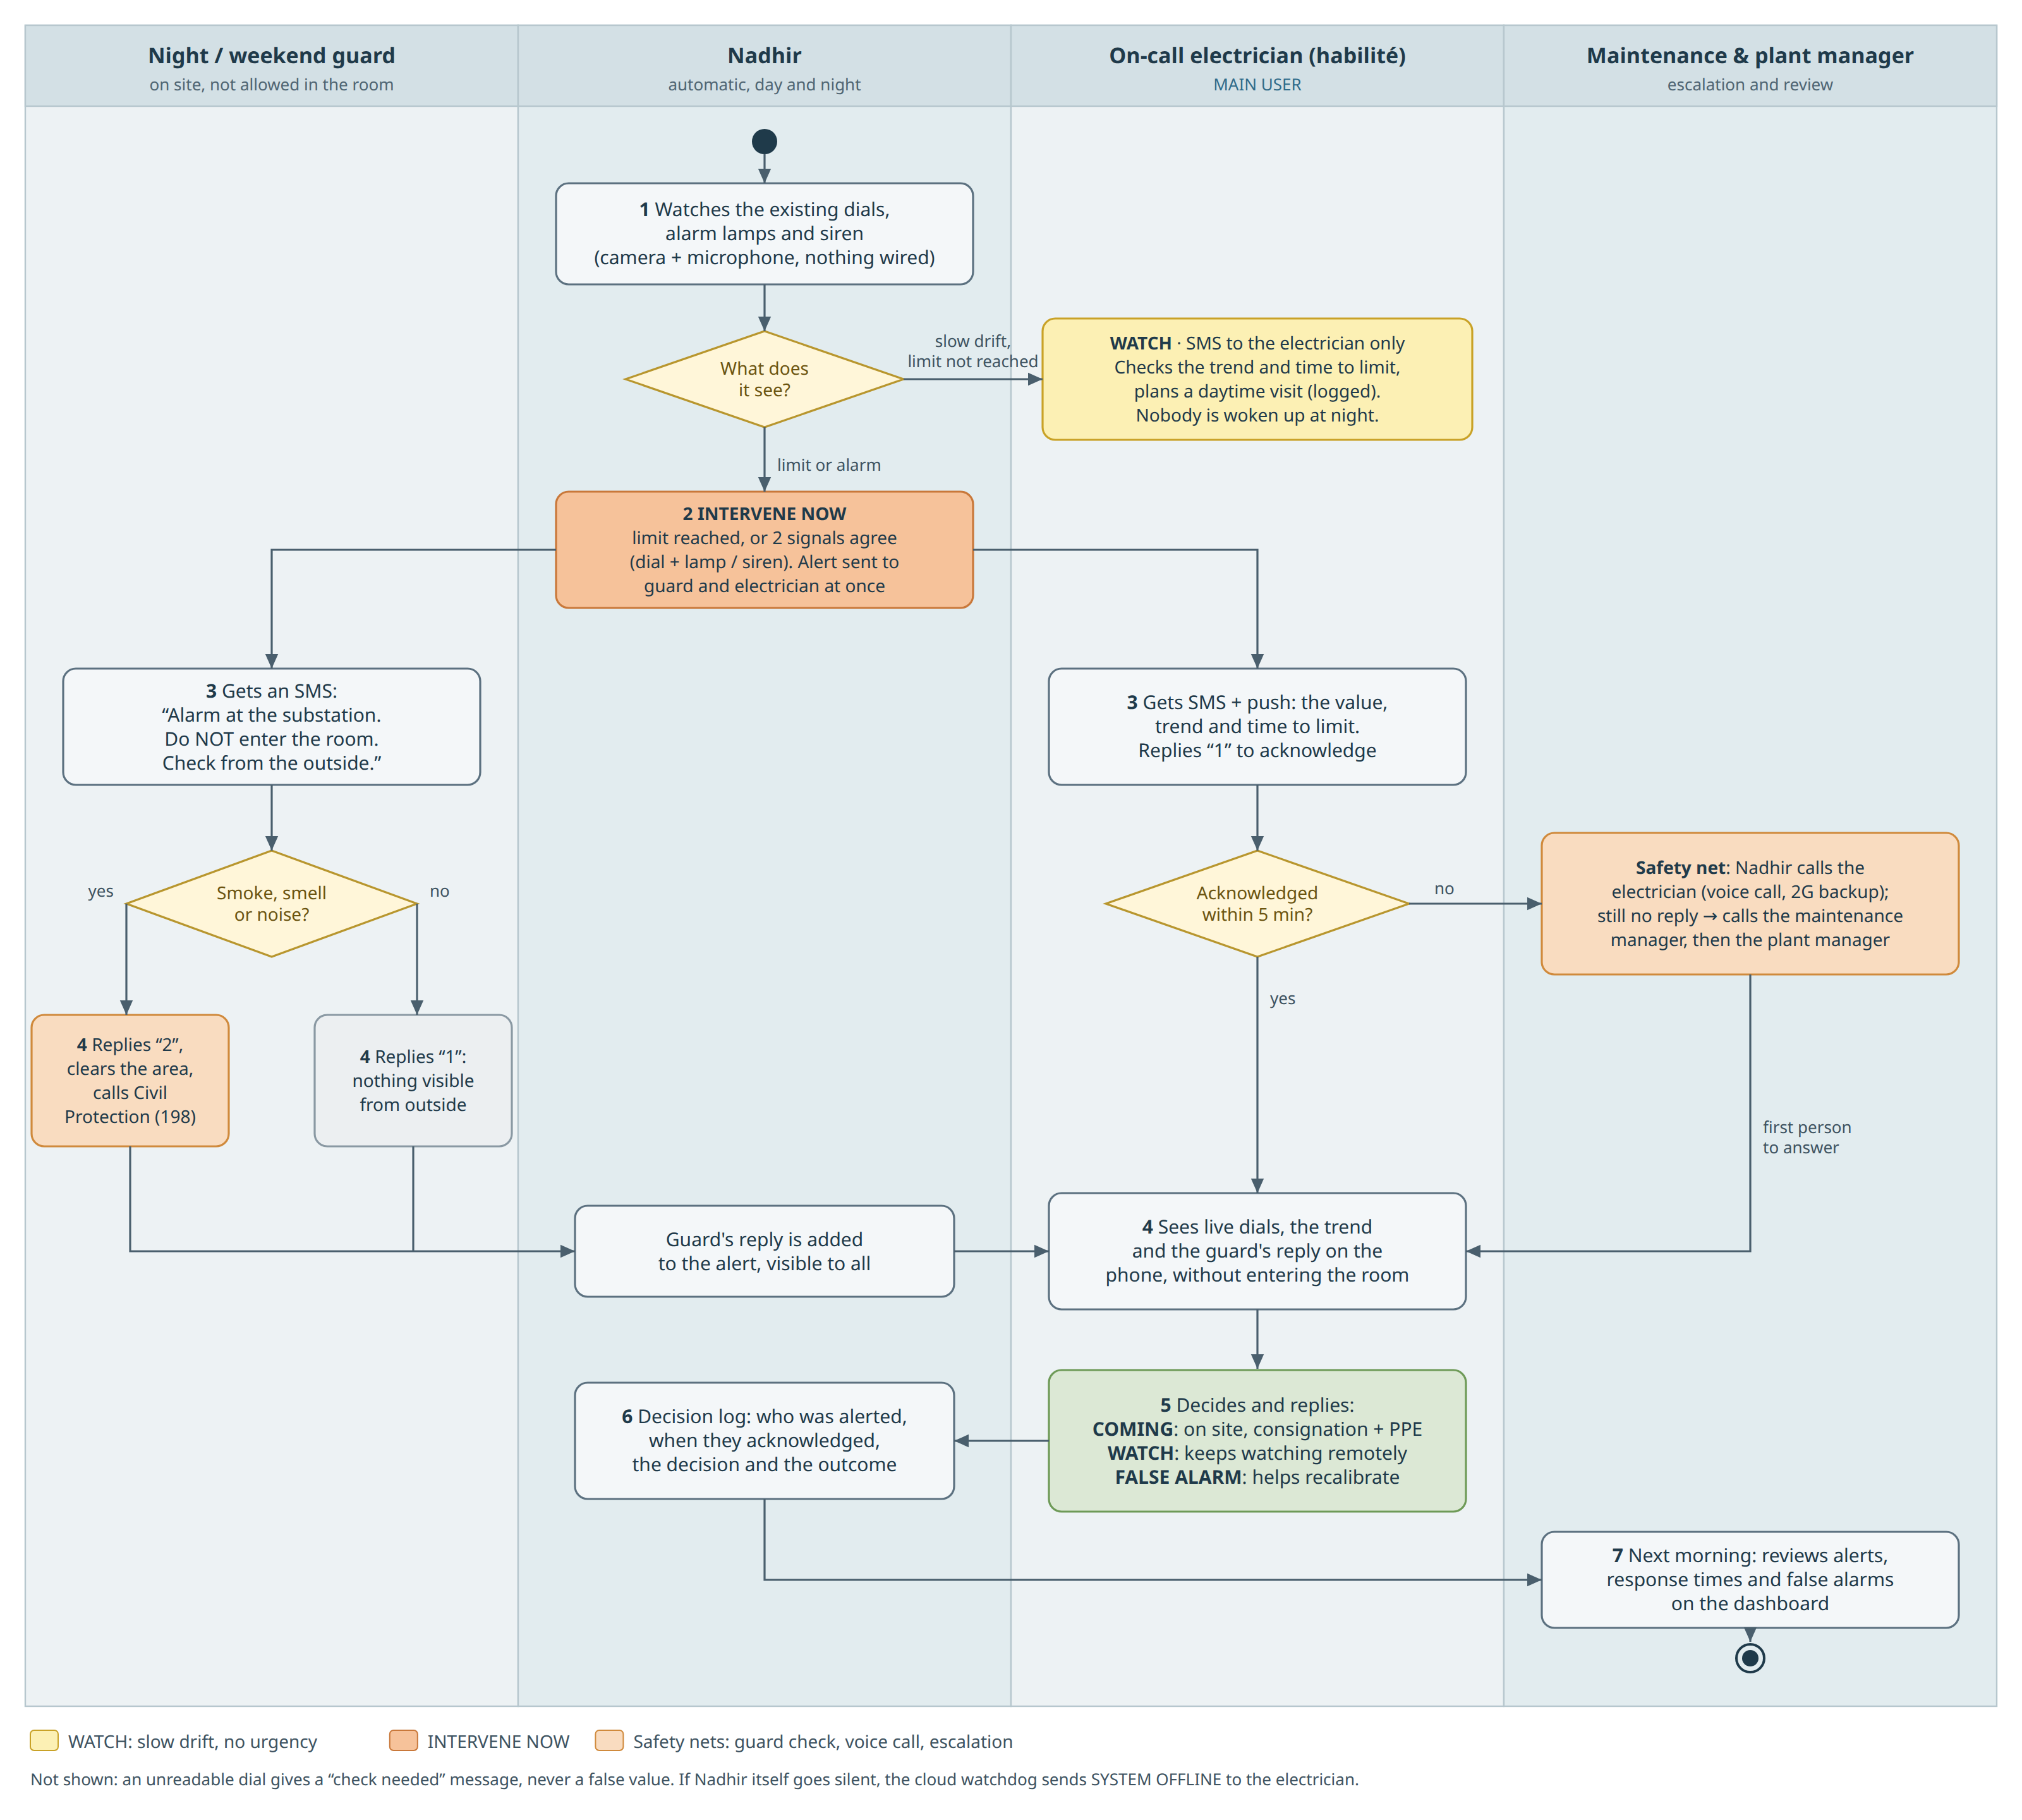
\includegraphics[width=\linewidth]{nadhir-user-journey.png}

\vspace{-2pt}
\textbf{User journey: an alarm on a night with the factory empty.}
Nadhir watches the existing dials, lamps and siren continuously and decides locally on a small on-site computer, so detection keeps working without internet.
A slow drift sends a WATCH SMS to the electrician only, and nobody is woken up for it.
A limit reached, or two signals agreeing, sends INTERVENE NOW to the guard and the electrician at once.
The guard checks from outside the room without entering and replies by SMS; the reply is shared with everyone on the alert.
The electrician acknowledges, sees the live values, the trend and the guard's report on their phone, and decides whether to come on site (with consignation and PPE), keep watching remotely, or mark a false alarm.
If nobody acknowledges within 5 minutes, Nadhir calls and then escalates to the managers.
Every step is logged and reviewed the next morning. If the connection drops, readings are stored on the box and synchronised when it returns, and a cloud watchdog raises SYSTEM OFFLINE if the box stops sending its heartbeat. Only readings and alerts leave the site, never the video.

\textbf{Key benefit:} the existing local dials, lamps and siren become a connected system that spots abnormal trends early and reaches the maintenance team even when the factory is unattended, without modifying the electrical installation.

\newpage
%==================================================================
\section{Feasibility}

\subhead{Tools and technologies}

\noindent\begin{tabularx}{\linewidth}{>{\bfseries\raggedright\arraybackslash}p{3.1cm} Y}
\rowcolor{head}\textbf{Building block} & \textbf{Choice} \\
Sensing & Infrared night-vision camera and USB microphone, fixed outside the danger zone; they only watch and listen. \\
\rowcolor{soft}Edge computer & Raspberry Pi class mini-computer running Python: reading, limits, trends and alert decision run on site, without internet; readings are buffered locally and synchronised automatically when 4G returns. \\
Dial and lamp reading & OpenCV: locate each dial, measure the needle angle, convert it to a value with a one-time calibration and a confidence score; lamps are read by colour and brightness. \\
\rowcolor{soft}Siren detection & Python spectrum analysis (frequency band + beep rhythm), calibrated on the real siren of each site. \\
Communication & 4G modem (data, SMS) as the main channel; 2G GSM module on a second operator for backup SMS and voice calls with a pre-recorded message. \\
\rowcolor{soft}Platform & PostgreSQL (readings, alerts, decisions, history), web dashboard, push notifications, heartbeat watchdog. \\
Resilience & UPS battery for power cuts; heartbeat to a cloud watchdog that sends SYSTEM OFFLINE when the box goes silent; the Pi's built-in hardware watchdog restarts a frozen box. \\
\rowcolor{soft}Security & Outbound-only encrypted connection, no open ports on site, no video sent off site. \\
\end{tabularx}

\subhead{Team skills}

\noindent\begin{tabularx}{\linewidth}{Y Y Y}
\rowcolor{head}\textbf{Already have} & \textbf{Need to develop} & \textbf{How we close the gap} \\
Programming and software development (Python, web) & MT/BT substation operation and safe camera placement & The technical directors interviewed in Phase 1 act as advisors; installation is always done by a \emph{habilité} \\
\rowcolor{soft}Databases and dashboard development & Embedded / IoT: Raspberry Pi, 4G and GSM modems & Bench build in the first weeks of Phase 3, starting from the modules' documented AT-command examples \\
Data analysis and machine learning & Computer vision for dial reading & Test bench of printed dials and photographed gauges before any site visit \\
\rowcolor{soft}System design and problem-solving & Audio processing for siren detection; industrial cybersecurity & Recorded siren + background noise for tuning; secure-by-default design (outbound only, no video) \\
\end{tabularx}

\subhead{Required resources}

\noindent\begin{tabularx}{\linewidth}{>{\bfseries}p{2.3cm} Y}
\rowcolor{head}\textbf{Resource} & \textbf{What we need} \\
Budget &
Prototype box, estimated at about \textbf{800 TND} one-time: mini-computer + memory card + power supply ($\approx$300), infrared camera ($\approx$150), 4G modem ($\approx$120), UPS module + batteries ($\approx$100), enclosure, mounts and cables ($\approx$60), 2G GSM module ($\approx$40), USB microphone ($\approx$30). Running cost: two SIM cards with SMS/data credit, about 20--30 TND per month; cloud on a free or student tier for the prototype. \emph{Estimates from typical local retail prices, to be confirmed with suppliers.} \\
\rowcolor{soft}Hardware & The components above, plus a printed-dial test bench for development. \\
Data & Photos and videos of real dials and lamps (day and night), recordings of the real siren and the background noise, past alarm logs and maintenance records. \\
\rowcolor{soft}Partners & A pilot factory and its \emph{habilité} electricians (from the Phase 1 interviews); telecom operators to confirm 4G and 2G coverage at the site. \\
\end{tabularx}

%==================================================================
\section{Risks}
\vspace{2pt}

\noindent\begin{tabularx}{\linewidth}{>{\raggedright\arraybackslash}p{4.2cm} >{\centering\arraybackslash}p{2.1cm} Y}
\rowcolor{head}\textbf{Risk} & \textbf{Likelihood} & \textbf{How we handle it} \\
\textbf{1. Reading or detection errors}: a dial misread (glare, darkness, angle) or the siren confused with factory noise &
\cellcolor{high}\textbf{High} &
Fixed mount with infrared light; one-time calibration per dial; a confidence score on each reading and a ``check needed'' message instead of a false value. The siren must match both frequency band and beep rhythm, calibrated on site. INTERVENE NOW needs two agreeing signals, and every ``false alarm'' reply is used to recalibrate. \\
\textbf{2. No access to a real substation} for photos, siren recordings and a pilot &
\cellcolor{med}\textbf{Medium} &
Ask the technical directors interviewed in Phase 1 for a recording session and a pilot site, with a \emph{habilité} present. Fallback: a test bench with printed dials, a recorded siren and simulated drifts, so development does not wait for site access. \\
\textbf{3. Nadhir itself fails or goes offline} (power cut, frozen software, network loss) &
\cellcolor{med}\textbf{Medium} &
UPS battery; local storage of readings; 2G backup on a different operator from the 4G SIM, so one cell outage cannot cut both; hardware watchdog restart; cloud heartbeat that sends SYSTEM OFFLINE to the electrician if the box goes silent. \\
\end{tabularx}

%==================================================================
\section{Link to Phase 1}

\textbf{Phase 1 problem.} Transformer substations in Tunisian factories already have sensors and alarms, but the warning stays trapped in a room nobody is watching, so at night, on weekends or during shutdowns a slow, catchable drift can grow unseen into a threat to the plant and the people around it.

\vspace{2pt}
\noindent\begin{tabularx}{\linewidth}{Y Y}
\rowcolor{head}\textbf{Validated need (Phase 1)} & \textbf{Part of the solution that answers it} \\
Detection already exists but stays local and passive: the missing piece is the last mile from sensor to human. \emph{(Needs assessment §1, §5; technical-director interviews)} &
\textbf{Touch-nothing monitoring}: camera and microphone read the existing dials, lamps and siren and carry the warning off site, with no wiring and nothing to re-certify. \\
\rowcolor{soft}Faults develop slowly (overheating, degrading oil) and can be caught early if someone sees the drift. \emph{(Needs assessment §1)} &
\textbf{Trend detection}: WATCH level with the trend and the time left before the limit. \\
Once a fault starts there is no fast way to intervene, especially when the factory is unattended. \emph{(Technician interview; technical-director interviews)} &
\textbf{INTERVENE NOW} sent to the electrician and the guard at once, with voice call and escalation if nobody answers in 5 minutes. \\
\rowcolor{soft}Guards and floor workers cannot enter the room or verify a warning sign, and do not know whether anyone is watching. \emph{(Needs assessment §2c--d; technician interview)} &
\textbf{Guard role in the journey}: a safe outside check, a one-digit SMS reply shared with everyone on the alert, never entering the room. \\
Existing ERP/CMMS maintenance modules are too complex for floor and night staff, so they go unused. \emph{(Industrial-organization expert interview)} &
\textbf{Zero-app alerting}: plain SMS and voice calls for the guard; the dashboard is only for the electrician and the managers. \\
\rowcolor{soft}Current measures meet the STEG minimum rather than providing real monitoring; standards expect ongoing monitoring with traceability. \emph{(Technician interview; needs assessment §5, ISO 45001)} &
\textbf{Decision log} and morning review, plus \textbf{self-monitoring} so that a silent box is never mistaken for a normal situation. \\
A missed alert means damage and downtime, so the warning must still arrive when one channel fails. \emph{(Needs assessment §4)} &
\textbf{4G + 2G backup} on two operators, UPS battery and cloud watchdog. \\
\end{tabularx}

\end{document}
